\chapter{Project}
\section{Project Flow }
\begin{enumerate}
    \item Importing Required Libraries.
        \subitem os 
        \subitem random
        \subitem sqlite3
        \subitem time
        \subitem tkinter
        \subitem deepcopy
        \subitem partial
        \subitem PIL
        \subitem font
        \subitem pyglet
    \item Splash Page will appear.
    \item First Screen having asking Player's name and Option of Play as well as Link to the Developers Page will show.
    \item Second Screen having board of game.
    \item Then Player will play.
    \item Result Screen will be displayed in which game result, option of play game again and exit option. 
\end{enumerate}

\section{Program}
\lstinputlisting[language=Python,style=mystyle, label=chapters/code/tic tac toe.py]{chapters/code/tic tac toe.py}

\section{Output}

\hspace{14pt}
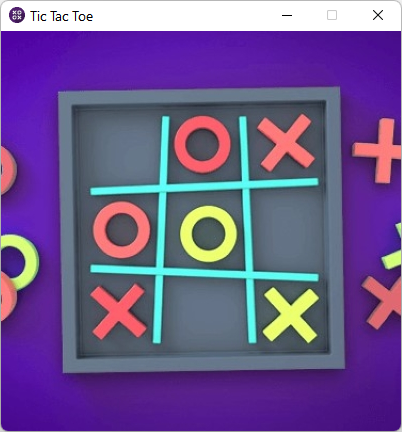
\includegraphics[width=8cm, height=9cm]{figures/splash_page.png}
\hfill
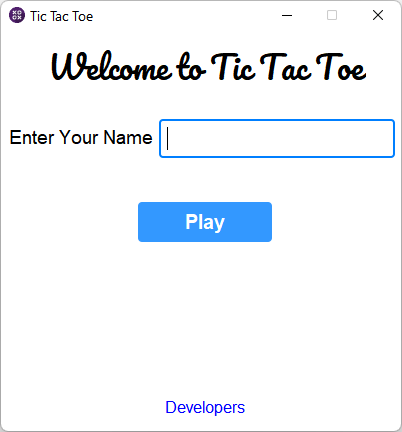
\includegraphics[width=8cm, height=9cm]{figures/first_screen.png}

\vspace{15pt}

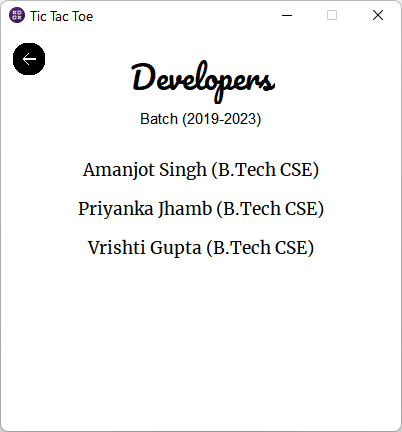
\includegraphics[width=8cm, height=9cm]{figures/developers_page.png}
\hfill
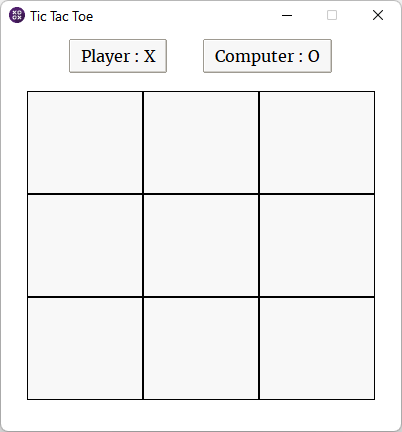
\includegraphics[width=8cm, height=9cm]{figures/GameBoard_page.png}

\vspace{10pt}

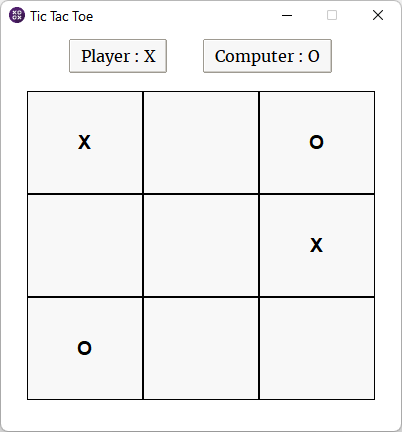
\includegraphics[height=8cm, width=8cm]{figures/GameBoard_page2.png}
\hfill
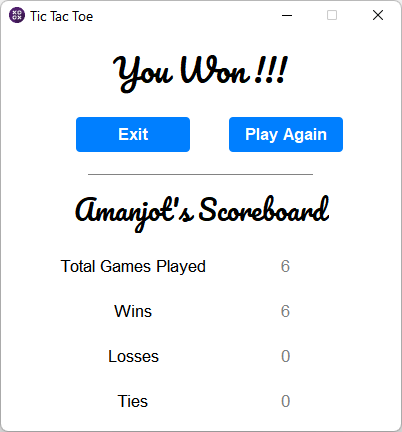
\includegraphics[height=8cm, width=8cm]{figures/Result_page_player_win.png}

\vspace{10pt}

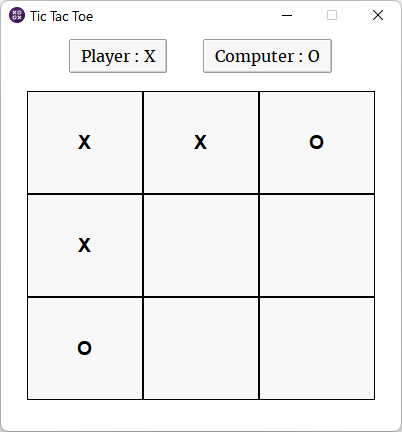
\includegraphics[height=8cm, width=8cm]{figures/GameBoard_page3.png}
\hfill
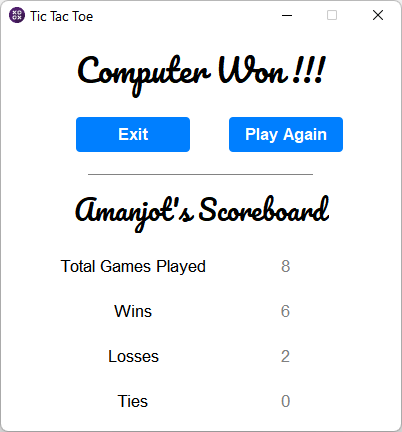
\includegraphics[height=8cm, width=8cm]{figures/Result_page_computer_win.png}

\vspace{15pt}
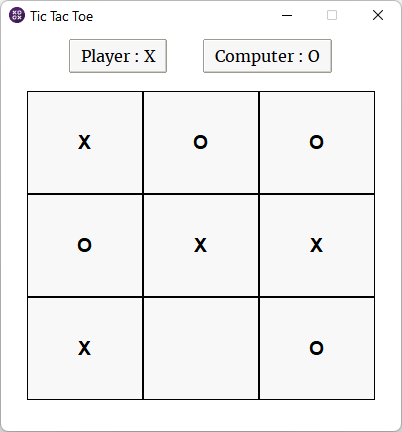
\includegraphics[height=8cm, width=8cm]{figures/GameBoard_page_tie.png}
\hfill
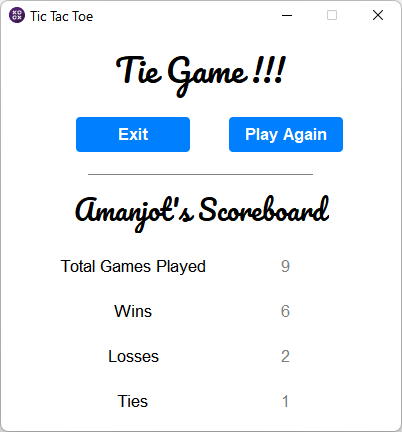
\includegraphics[height=8cm, width=8cm]{figures/Result_page_tie.png}
